\RequirePackage{fix-cm}
\documentclass[smallcondensed,natbib,nospthms]{svjour3}
\usepackage[T1]{fontenc}
\usepackage[utf8]{inputenc}
\usepackage{lmodern}
\usepackage{amsmath,amssymb}
\usepackage{booktabs,enumitem,graphicx,flafter,microtype,multirow}
\usepackage[section]{placeins}
\usepackage{tabularx,xcolor,xurl}
\usepackage[hidelinks]{hyperref}
\usepackage[nameinlink,noabbrev]{cleveref}
\setcitestyle{numbers,square,comma}
\providecommand{\bibcommenthead}{}
\hypersetup{pdftitle={Correction-Aware Data Admission},pdfauthor={Liang Hanghao; Xuan Wentao; Chen Qile; Peng Peng},pdfsubject={Data integrity, candidate-bound authorization, and field-level provenance}}
\setlength{\emergencystretch}{2em}
\newcommand{\system}{\textsc{Auto-Decte}}
\newcommand{\code}[1]{\nolinkurl{#1}}
\newcommand{\eqc}{\mathrel{=_{\mathrm{json}}}}
\newcommand{\neqc}{\mathrel{\neq_{\mathrm{json}}}}
\journalname{Journal of Intelligent Information Systems}
\begin{document}
\title{Correction-Aware Data Admission: Candidate-Bound Authorization and Field-Level Provenance for AI-Derived Updates}
\titlerunning{Correction-Aware Data Admission}
\author{\mbox{Liang Hanghao} \and \mbox{Xuan Wentao} \and \mbox{Chen Qile} \and \mbox{Peng Peng}}
\authorrunning{Liang Hanghao et al.}
\institute{Liang Hanghao \and Xuan Wentao \and Chen Qile \and Peng Peng \at
College of Computer Science and Electronic Engineering, Hunan University, Lushan South Road, Yuelu District, Changsha 410082, China\\
\email{hnu16pp@hnu.edu.cn} (Peng Peng, corresponding author)}
\date{}
\maketitle
\begin{abstract}
Human-reviewed AI-derived updates in intelligent information systems can produce identical authoritative values despite different machine proposals and authorizations. Correction must preserve what the machine proposed while recording the value a reviewer authorized. Even equal-valued candidates with equivalent retained context can be distinct authorization targets. We specify a correction-aware admission relation that binds review to an exact persisted candidate and an explicit authorized value. It checks predecessor freshness and atomically creates a complete successor with total field-level sources. Five paired histories establish class-wise irredundancy of failure-distinguishing information classes in the declared observation model. A Python/SQLite realization connects the relation to bounded Alloy analysis, formal--concrete projections, and a 35-case fault catalogue. In a policy comparison, an exact-binding event journal and the relational reference agree on all 165 corresponding cases. A context journal accepts 15 equal-valued substitutions that satisfy its value/context policy but violate instance authorization; both exact-binding mechanisms reject them. A server-held review-session gate rejects nine request substitutions accepted by the original confirmation path, while three display-only substitutions remain admissible in both paths. Current-version workloads characterize admission, reverse-trace, and storage costs. Together, the results establish an executable relation that preserves corrected proposal histories, enforces instance-specific authorization across two storage designs, and makes each committed field's authorization and source queryable.
\keywords{data integrity \and data provenance \and human authorization \and AI-assisted data acquisition \and transactional admission \and relational verification}
\end{abstract}

\section{Introduction}
\label{sec:introduction}

Intelligent information systems combine machine-produced information with persistent operational records. In document intelligence and human-in-the-loop data curation, reviewers may authorize a correction before a proposed value enters those records. The final authoritative value cannot recover which proposal was reviewed, what value was authorized, or which predecessor and field sources were retained. The problem is to preserve that authorization history in a queryable authoritative state.

Consider quantity 90. A recognizer proposes 100, and a reviewer authorizes 101. Correction should retain both the machine proposal and human-authorized value; an unchanged batch-code field should retain its exact earlier source. Proposal origin and value authority are different roles, including when
\begin{equation}
x_c\neq x_a.
\label{eq:intro-correction}
\end{equation}
Overwriting the original proposal would instead attribute the corrected value to the machine.

Candidate identity introduces a second distinction. Two persisted extraction attempts can share the proposed value, record, field, evidence, expected version, and other retained review context. They remain different instances. Content/context equivalence does not make an unreviewed substitute the same authorization target. Equal-valued candidate substitution isolates this difference.

Transactions, optimistic validation, provenance, and version-specific human approval provide established foundations \citep{gray1981transaction,kung1981occ,moreau2013provdm,mershad2015approval}. We specify a correction-aware admission relation for this review-to-state boundary and characterize the information that distinguishes its failure families. The relation connects
\begin{equation}
\begin{aligned}
\textit{exact candidate}
&\rightarrow\textit{candidate-bound authorization}\\
&\rightarrow\textit{explicit authorized value}\\
&\rightarrow\textit{fresh authoritative predecessor}\\
&\rightarrow\textit{complete successor and total field sources}.
\end{aligned}
\label{eq:admission-chain}
\end{equation}
Authorization permits the committed value; the candidate remains historical evidence. One transaction creates new transitions for changed fields and preserves exact sources for unchanged fields.

We realize the relation in \system{}, a Python/SQLite service, and make three contributions:
\begin{enumerate}[label=\textbf{C\arabic*:},leftmargin=*]
\item \textbf{We define correction-aware admission and characterize its failure-distinguishing information.} Five paired histories establish class-wise irredundancy of candidate identity/context, value roles, freshness, successor completeness, and field-source attribution in the declared observation model.
\item \textbf{We implement the relation and connect specification to persisted behavior.} Bounded Alloy analysis, selected formal--concrete projections, and fault injection examine transaction bindings, atomic successors, and source evolution.
\item \textbf{We isolate the authorization-policy difference and examine its operational boundary.} Equal-valued substitutions separate context from instance approval; session controls test review-to-confirmation consistency; current-version workloads characterize admission and provenance costs.
\end{enumerate}

The exact-binding journal and relational reference agree on all 165 corresponding cases. The context journal accepts 15 equal-valued substitutions permitted by its value/context policy; the exact mechanisms reject them under instance authorization. Evaluating both policies on their own terms separates the required authorization target from storage design.

A confirmation request can disagree with recorded review intent even when its transaction is internally consistent. Server-held session binding examines that transfer, and display controls locate the presentation boundary. \Cref{fig:admission-workflow} summarizes the relation from reviewed instance through Correction to field sources.

\begin{figure}[!htbp]
\centering
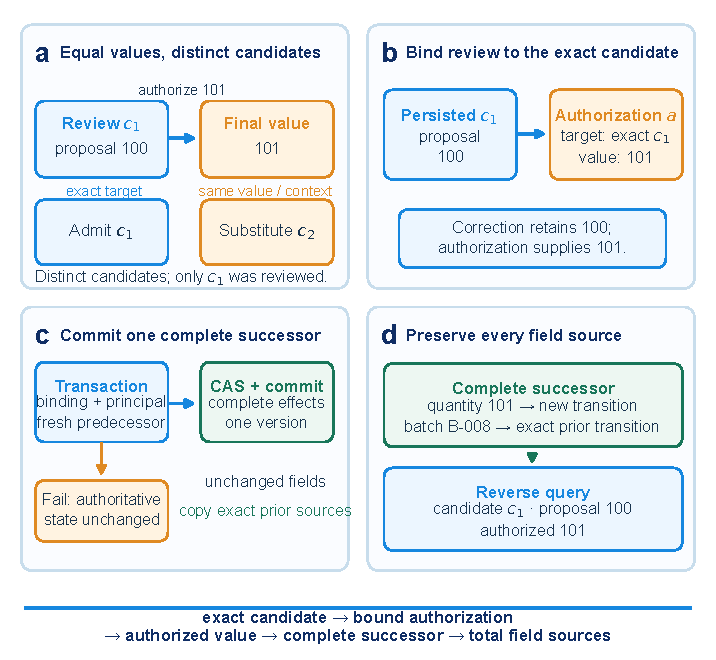
\includegraphics[width=0.975\textwidth]{figures/refined/figure-1-admission-workflow.pdf}
\caption{The admission relation preserves both the reviewed instance and the original proposal through Correction. (a) Equal-valued candidates remain distinct authorization targets; (b) the authorized correction retains the proposal; (c) failed admission leaves authoritative state unchanged; (d) changed and unchanged fields retain their respective sources. Values illustrate a constructed example. Diagram preparation assisted by OpenAI Codex; image-generation prototype use is disclosed in Statements and Declarations}
\label{fig:admission-workflow}
\end{figure}

\section{Related work}
\label{sec:related}

\subsection{Transactions, update provenance, and event histories}

Transactions provide atomic, durable, consistency-preserving state transformations \citep{gray1981transaction}. Optimistic concurrency control validates conflicting work before installing effects \citep{kung1981occ}. Together, they support complete successors and commit-time predecessor checks.

Why-, how-, and where-provenance explain contributing data, derivations, and source locations \citep{buneman2001whywhere,cheney2009provenance}. Curated-database provenance also records edits and copies across versions. In particular, \citet{buneman2006curated} explicitly link unchanged data to the preceding version and support source, history, and modification queries. Exact source preservation is therefore an established provenance technique.

Reenactment recovers multi-version transaction provenance from update histories, logs, and prior versions \citep{arab2018reenactment}. PROV-DM supplies entities, activities, agents, derivation, and responsibility \citep{moreau2013provdm}. Both support richer application histories when the necessary objects are recorded.

Event sourcing reconstructs state from recorded events \citep{fowler2005eventsourcing}. An event schema can retain original proposals, corrected values, reviews, versions, and sources. Its validation policy determines whether authorization targets equivalent content or a particular proposal instance. These foundations support the correction-aware relation studied here: admission checks the reviewed candidate, authorized value, predecessor, and every field's source together. E1 uses the same journal design and transactional mechanisms while changing the reviewed-candidate link; the relational reference checks agreement across representations.

\subsection{Human approval, correction, and data curation}

Human-controlled integrity transitions have substantial precedents. Clark--Wilson combines well-formed transactions, authenticated execution relationships, separation of duty, and reconstructible audit records \citep{clark1987integrity}. In collaborative databases, \citet{mershad2015approval} persist cell versions pending principal-investigator approval. The reviewer selects historical records by cell identifier and timestamp. This already provides version-specific content approval, beyond permissions based on the updater's identity.

Interactive cleaning also separates system suggestions from human judgments. Guided Data Repair maintains candidate cell repairs and lets users confirm, reject, retain the current value, or supply a replacement \citep{yakout2011guided}. Falcon turns user corrections into candidate update rules for validation \citep{he2016falcon}. Its closed-rule analysis recognizes that rules with identical effects on the current data can differ in semantic validity. Thus human correction and the distinction between equal results and different semantics precede this work. Wrangler further provides editable transformation histories, previews, and reusable scripts \citep{kandel2011wrangler}.

DBWiki combines fine-grained node identities, version history, atomic edits, and provenance queries for collaborative curation \citep{buneman2011dbwiki}. These systems already provide components of a proposal--review--update history. The relation studied here connects those parts at field-level admission: retain the original $x_c$, bind the human-authorized $x_a$ to the exact reviewed candidate, revalidate the authoritative predecessor, and atomically install a complete successor with total sources. Our paired-history analysis characterizes the information distinctions of this specified relation. The comparator then isolates whether equal-valued, context-equivalent candidates are interchangeable under two explicit authorization policies.

\subsection{Governed AI state and persistent memory}

Continuity Kernel is a close neighboring activation contract \citep{he2026continuity}. It binds exact proposal identity, predecessor, pre-state authority, signed approver evidence, and lineage to an atomic complete accepted unit. It supports human interaction during preparation and several storage realizations. We build on these activation principles to specify the field-level Correction relation, retaining proposed and authorized values with exact changed/unchanged sources, and analyze its failure-distinguishing observations.

MemTxn separates source-supported update admission, temporal visibility, and complete-state recovery \citep{cui2026memtxn}. MutMem binds signed old/new retrieval-weight mutations to memory identity, provenance, signer epochs, and predecessor continuity \citep{saidi2026mutmem}. LatticeMind manages claim status, conflict, supersession, and provenance \citep{zhou2026latticemind}. Stored Is Not Supported governs assertion release from an authenticated accepted head through typed provenance \citep{he2026stored}. Together, these accounts cover activation, mutation, and later use of persistent state. All five are currently preprints, and their representations may also encode the correction-aware field relation. Here we study that relation through its failure-distinguishing observations and controlled policy comparison.

\subsection{Binding and executable specification}

Security binding provides related concepts at another semantic layer. OAuth DPoP binds proof-of-possession to request method and URI \citep{fett2023dpop}; HTTP Message Signatures cover components selected by an application profile \citep{backman2024signatures}. OWASP transaction-authorization guidance requires server-controlled approval data, invalidation after relevant changes, and a final authorization gate \citep{owaspTransactionAuthorization}. E2 applies this established discipline to transferring a recorded candidate review into confirmation, with separate request and display controls.

Alloy and Kodkod support bounded relational specification and model finding \citep{jackson2002alloy,torlak2007kodkod}. TestEra connects specifications to execution through concretization and output abstraction \citep{marinov2001testera}. We use these methods to check an application contract and selected persisted-state projections. The paired histories show which distinctions disappear when information is omitted; model checks and persisted-state projections test the encoded contract.

\section{Authoritative-state admission contract}
\label{sec:contract}

\subsection{Candidate, authorization, and authoritative state}


Correction-aware admission links an untrusted persisted candidate $c$, attributable authorization $a$, and authoritative pre-state $\Sigma_v$:
\begin{equation}
\operatorname{Admit}(c,a,\Sigma_v)=\Sigma_{v+1}.
\label{eq:admit}
\end{equation}
The candidate stays non-authoritative historical evidence. Proposal origin, value authority, and committed value remain distinct roles.

Let $r$ be a record with a nonempty authoritative field set $F_r$. Its committed state $\Sigma_v$ contains a total value map $V_v:F_r\rightarrow X$ and a total source map $S_v:F_r\rightarrow T$, where $T$ is the set of durable fact transitions. A machine candidate for field $f$ is
\begin{equation}
c=\langle r,f,e,v_{\mathrm{exp}},x_c,p,c_{\mathrm{id}}\rangle,
\label{eq:candidate}
\end{equation}
where $e$ is persisted evidence, $v_{\mathrm{exp}}$ is the expected current version, $x_c$ is the machine proposal, and $p$ identifies its producer. The identity $c_{\mathrm{id}}$ distinguishes exact persisted candidate instances even when proposal values and retained review context agree.


Evidence identity combines a content digest and canonical record/field locator:
\begin{equation}
EID(e)=\langle H(\mathrm{bytes}(e)),L(r,f,u,\kappa)\rangle.
\label{eq:evidence}
\end{equation}
Here $H$ is SHA-256, and $L$ contains the owner record, field, normalized storage-relative URI $u$, locator version, and optional crop $\kappa$. Alloy abstracts content and locators as primitive domains. Identity uniqueness in its scopes relies on collision resistance and canonicalization/store integrity in the implementation (Online Resource 1, Section S2).

An attributable authorization is
\begin{equation}
a=\langle c_{\mathrm{id}},x_a,q\rangle,
\label{eq:authorization}
\end{equation}
where $q$ is an authorized human principal and $x_a$ is the value explicitly permitted to enter the record. The dual-value semantics are
\begin{align}
\operatorname{proposal}(c)&=x_c, &
\operatorname{authorize}(a)&=x_a,\nonumber\\
\operatorname{commit}(\Sigma_{v+1},f)&=x_a, &
\operatorname{origin}(\Sigma_{v+1},f)&=c.
\label{eq:dual-value}
\end{align}
Accept has $x_c\eqc x_a$. Correction has $x_c\neqc x_a$; the candidate remains unchanged and the committed value derives its authority from $a$. Here $\operatorname{origin}$ identifies the retained proposal, not the authority for a corrected value.


\paragraph{Canonical value equality}
Write $x\eqc y$ when sorted-key, whitespace-minimal JSON serializations agree. This distinguishes $2$ from $2.0$ and $1$ from \code{true}, although Python equality does not. Change detection, value checks, tracing, the independent oracle, and projection use this relation. \Cref{sec:conformance} reports the cross-layer repair.

\subsection{History, observations, and outcomes}

An authority-relevant history is
\begin{equation}
h=\Sigma_0\xrightarrow{e_1}\Sigma_1\xrightarrow{e_2}\cdots\xrightarrow{e_n}\Sigma_n,
\end{equation}
where events may persist evidence or candidates, record review and authorization, attempt admission, commit or stutter, and reconstruct a reverse trace. The abstraction describes semantic information rather than requiring particular table or column names.

Equal-valued substitution exposes one missing distinction. Extending the analysis across the admission relation yields five information classes for the modeled failures:
\begin{equation}
\mathcal D=\{D_C,D_V,D_F,D_B,D_S\},
\label{eq:distinction-basis}
\end{equation}
where $D_C$ is candidate identity and context, $D_V$ is dual-value attribution, $D_F$ is freshness, $D_B$ is batch/successor completeness, and $D_S$ is total source attribution. For $I\subseteq\mathcal D$, $\pi_I(h)$ retains only the information classes in $I$. A certificate or stable handle may implement this identity, provided distinct persisted instances remain distinguishable despite equivalent values and retained context. Freshness may likewise use a version, state hash, epoch, or comparable discriminator.

To make ``retains'' precise, let $\operatorname{obs}_d(h)$ be the observation function for class $d$ and define
\begin{equation}
\pi_I(h)=\langle\operatorname{obs}_d(h)\rangle_{d\in I}.
\label{eq:observation-projection}
\end{equation}
The functions are logical projections, not claims that a database must store five physically separate objects. A certificate can co-locate several classes. In a projection, however, a content address is treated as an opaque equality-preserving handle: its preimage is not available as a side channel. This prevents a nominally omitted value or version from being recovered merely because the concrete certificate hash covers it. The complete observation functions are given in Online Resource 1, Section S2.

The full-history authority-outcome label is
\begin{equation}
O(h)=\langle status,successor,trace\rangle,
\label{eq:outcome}
\end{equation}
where $status$ is admissible, inadmissible, or failed/stuttering; $successor$ classifies the authoritative post-state or its absence; and $trace$ is complete, incomplete, ambiguous, or unavailable. This is the normative label assigned from the full history, not an additional input available to a mechanism restricted to $\pi_I$. A binary accept/reject label is insufficient because value-identical successors may differ in source completeness.

An observation set $I$ fails to distinguish a failure family when there exist a safe history $h_s$ and unsafe history $h_u$ such that
\begin{equation}
O(h_s)\neq O(h_u)
\quad\land\quad
\pi_I(h_s)=\pi_I(h_u).
\label{eq:indistinguishable}
\end{equation}
Any admission decision based only on that reduced observation cannot separate the pair.


The executable histories contain candidate and authorization registries, declared items, expected and observed versions, a connected commit sequence, endpoint maps, and transition sources. Projections and outcomes are derived from these relations. Schema fields determine total map domains; declared items determine required effects. Missing or conflicting sources remain failures in the domain. Online Resource 1, Section S2 gives the complete functions, finite tuple, and checker rules.

\subsection{Conditional failure-distinguishability characterization}

The five classes distinguish candidate substitution, false value attribution, stale replay, fragmented successors, and source ambiguity. Table~\ref{tab:distinctions} identifies a safe/unsafe pair for each class in the fixed observation basis.

\begin{table}[t]
\centering
\footnotesize
\caption{Failure-distinguishing information classes in the declared observation model.}
\label{tab:distinctions}
\begin{tabularx}{\textwidth}{@{}l>{\raggedright\arraybackslash}p{0.23\textwidth}>{\raggedright\arraybackslash}p{0.27\textwidth}>{\raggedright\arraybackslash}X@{}}
\toprule
Class & Safe/unsafe pair & Required distinction & Failure if omitted \\
\midrule
$D_C$ & exact candidate / equal-valued cross-context substitute & persisted candidate identity plus record, field, evidence, and producer context & candidate substitution \\
$D_V$ & preserved Correction / erased or false role attribution with the candidate unchanged & separate machine proposal $x_c$, human-authorized value $x_a$, committed value, and role relation & correction erasure or false machine attribution \\
$D_F$ & current authorization / same authorization after supersession & commit-time freshness discriminator tied to the observed pre-state & stale replay \\
$D_B$ & one atomic commit / two connected commits with the same final values & actual per-step effects and one atomic successor & fragmented successor \\
$D_S$ & total trace / equal-valued successor with missing or conflicting source & total per-field source relation and exact unchanged-source copy-forward & source ambiguity \\
\bottomrule
\end{tabularx}
\end{table}

\paragraph{Proposition 1 (conditional failure distinguishability)}
For each information class $d_i\in\mathcal D$, the declared failure model contains a safe history and a corresponding unsafe history whose authority outcomes differ but whose projections become equal when $d_i$ is omitted. Consequently, an admission mechanism that observes only $\mathcal D\setminus\{d_i\}$ cannot distinguish the paired failure family under this model.

\paragraph{Proof sketch (by construction)}
For $D_C$, hold the value-role, temporal, batch, and source observations constant while changing non-temporal candidate context. For $D_V$, retain the same candidate, proposal value 100, and committed value 101, but falsely attribute the corrected value to the machine proposal. For $D_F$, change only the admission-entry freshness comparison. For $D_B$, compare one two-field commit with two connected single-field commits that reach the same final values and sources; the latter exposes an intermediate partial state. Effect domains and successor counts follow from these sequences. For $D_S$, remove one source anchor while retaining candidates, values, freshness, and the commit sequence. Each construction changes its selected observation coordinate and the derived outcome, while leaving the other four coordinates equal.

Thus, for every $d_i\in\mathcal D$, the constructed histories satisfy
\begin{equation}
\pi_{\mathcal D\setminus\{d_i\}}(h_s^{(i)})
=
\pi_{\mathcal D\setminus\{d_i\}}(h_u^{(i)})
\quad\text{and}\quad
O(h_s^{(i)})\neq O(h_u^{(i)}).
\label{eq:irredundancy}
\end{equation}
Any decision function of the reduced projection receives the same input for both histories and cannot assign both distinct required outcomes. This establishes the claimed conditional irredundancy.

The executable checker validates each complete $\widehat h$ and derives observations and outcomes from its relations; witnesses store neither. It checks domain validity, unequal outcomes, equal four-class projections, and unequal full projections. Schema fields define the total value/source domains, whereas declared item fields define the required effect domain.

The original $D_C$ pair changes record context while retaining the candidate handle, establishing irredundancy of the combined class. An additional pair fixes the two-candidate registry and every context/value component, then selects either the authorized candidate or the equal-valued alternative. It isolates candidate binding within this observation model. A single-field copy-forward control checks the distinction between schema and effect domains. Online Resource 1, Section S2 identifies the executable constructions and raw histories.

\paragraph{Scope of the result}
Proposition 1 establishes Eq.~\eqref{eq:irredundancy} for the declared failure, history, observation, and outcome model. Its scope is class-wise irredundancy, not universal minimality, schema uniqueness, or completeness over all admission failures. The checker validates the five class pairs, identity pair, and copy-forward control rather than arbitrary admissions. Separate Alloy checks examine the encoded assertions and conjunct-removal sensitivity in finite scopes.

\subsection{Batch admission relation}

A batch $B$ is a nonempty set of items sharing one target record, principal, expected pre-version, and successor. Under Full, item fields are unique. Let
\begin{equation}
\Delta(V_v,V_{v+1})=\{f\in F_r\mid V_v(f)\neqc V_{v+1}(f)\}.
\end{equation}
For a post-initial concrete admission,
\begin{equation}
\Delta(V_v,V_{v+1})=\{i.f\mid i\in B\}=\{t.f\mid t\in T_{v+1}\},
\label{eq:changed-fields}
\end{equation}
with one transition per item. At the first certificate-era version, the batch covers all of $F_r$, establishing total value and source domains. Deletion is outside the model.

For every $i\in B$, admission requires
\begin{align}
i.r &= r, & i.f&\in F_r,\nonumber\\
EID(i.e) &= EID(i.c.e), & i.v_{\mathrm{exp}}&=v,\nonumber\\
i.a.c_{\mathrm{id}}&=i.c.c_{\mathrm{id}}, & i.a.q&=q,\nonumber\\
i.x &\eqc i.a.x_a, & t_i.x&\eqc V_{v+1}(i.f)\eqc i.x.
\label{eq:item-bindings}
\end{align}
Together these instantiate the admission preconditions
\begin{equation}
\begin{aligned}
&\operatorname{Bind}(a,c)\land\operatorname{Fresh}(c,\Sigma_v)\land\operatorname{Authorized}(a)\\
&\qquad\land\operatorname{Complete}(\Sigma_{v+1})\land\operatorname{Attributed}(\Sigma_{v+1}).
\end{aligned}
\end{equation}

The successor is atomic: all admission-time decision, authorization, transition, version, source-map, and audit effects commit together, or authoritative state stutters. This does not require rollback of evidence, candidates, or review intent persisted before the admission attempt. For a changed field, $S_{v+1}(f)=t_i$. For an unchanged field, value and exact source are copied forward:
\begin{equation}
f\notin\Delta(V_v,V_{v+1})\Rightarrow
V_{v+1}(f)\eqc V_v(f)\land S_{v+1}(f)=S_v(f).
\label{eq:copy-forward}
\end{equation}
Alloy permits same-value admission for correspondence with the historical singleton model; concrete post-initial admissions require a value change. For submitted items $U$, the admitted batch is $B=\{i\in U\mid i.x\neqc V_v(i.f)\}$, with $B\neq\varnothing$. A mixed submission admits exactly $B$ and copies unchanged items' exact prior sources into the complete successor, creating no transition or authorization binding for $U\setminus B$. Thus Eq.~\eqref{eq:changed-fields} concerns admitted effects, not all submitted reviews. Recording renewed review or re-attribution without a value change requires a separate review-event path outside this contract; persisted candidate identity allows that path to distinguish equal-valued proposals.

\subsection{Operational properties and trust boundary}

\begin{table}[t]
\centering
\caption{Admission properties and their operational interpretation.}
\label{tab:properties}
\begin{tabularx}{\textwidth}{@{}l>{\raggedright\arraybackslash}p{0.29\textwidth}>{\raggedright\arraybackslash}X@{}}
\toprule
Property & Requirement & Operational interpretation \\
\midrule
P0 & Direct-write exclusion & Machine/candidate capability cannot change authoritative values, versions, sources, transitions, or authorizations. \\
P1 & Candidate non-substitutability & Authority refers to the same canonical persisted certificate, not merely an equal value or analogous candidate. \\
P2 & Context-bound admission & Record, field, persisted evidence content and locator, and expected version agree across the item and certificate. \\
P3 & Authorization integrity & The principal is allowed at the in-transaction policy check before the compare-and-swap, and the authorization names the exact certificate and explicit committed value; in-flight revocation semantics are stated in \cref{sec:authorization-timing}. \\
P4 & Freshness & The expected version equals the transactionally observed current version; stale or competing decisions fail closed. \\
P5 & Successor integrity & One atomic successor has an item--transition bijection, exact changed-field effects, and complete changed/unchanged framing. \\
P6 & Trace soundness & Each committed field resolves through its exact source transition to consistent authorization, certificate, evidence, producer, and version relations. \\
\bottomrule
\end{tabularx}
\end{table}


Model output and candidate-only callers are untrusted. The trusted base comprises the admission service, adapter, exercised transaction semantics, canonicalization and hashing, and principal policy. Host authentication, session integrity, and faithful review presentation are external assumptions. The confirmation API constructs its binding from caller-supplied candidate and value; the contract preserves that binding, not factual truth or protection from a compromised host.

\paragraph{Authorization timing and revocation}
\label{sec:authorization-timing}
The in-transaction principal check precedes compare-and-swap and authority writes. Revocation visible before the check causes zero-write rejection; a later overlapping revocation does not cancel an in-flight commit. This is commit-entry revalidation. Online Resource 1, Section S2 states the policy-lock and stronger-revocation boundaries.

\section{Bounded relational characterization}
\label{sec:alloy}

Relational analysis examines the contract's legal steps, preservation properties, and sensitivity to removing individual bindings. It complements the observation-level construction by making the admission predicates executable.

The Alloy model represents records, fields, ordered versions, evidence, candidates, certificates, principals, authorizations, transitions, and states. Once a record is authoritative, its value and source maps cover exactly its field domain. \code{MachineEvent} can extend candidate/evidence sets while framing authority (P0). \code{BatchAdmissionEvent} has a nonempty item set in one envelope. \code{TamperEvent} freezes values and source pointers while modifying transitions.

The base effect advances one version and applies item values and sources. Full adds unique fields, complete snapshot shape, preexisting certificate/evidence, contextual and authorization bindings, freshness, and an exact item--transition bijection. Separating these conjuncts permits controlled removal. Each ablation uses at least two items: one violates only the selected conjunct and another remains Full-valid. The reduced relation admits that set; Full rejects it with authoritative-state stutter.

Six legal commands exercise Accept, Correction, mixed batches, same-value admission, initial coverage, and singleton admission. Eleven ablations test encoded bindings. Three source attacks remove, replace, or duplicate an anchor after a legal prefix. Fourteen assertions per profile check framing, preservation, singleton correspondence, and trace conditions. The class-to-conjunct map and complete command descriptions are in Online Resource 1, Section S2.

The positive trace assertion requires a trace-complete predecessor and no stray successor transition. It checks admitted fields for one encoded step. Reachable initial and carry-forward witnesses establish a nonempty premise; removing post-state certificate binding changes UNSAT to SAT. Concrete tracing additionally validates predecessor prefixes. This distinguishes bounded preservation from the observation-level proposition.

Two scope profiles increase representative bounds from two records, three fields, six versions, and four states/events to three records, four fields, eight versions, and five states/events. Individual domain bounds remain fixed by deposited commands. SAT denotes a found witness; UNSAT denotes no counterexample within that command's finite scope \citep{jackson2002alloy,torlak2007kodkod}.

% Generated from the frozen r27 Alloy receipts.
% Source: formal/alloy/batch/command_manifest.tsv and formal/alloy/batch/raw-results/2026-09-11-trace-witness/command_results.json
% r27 extension: +1 positive trace-completeness assertion per profile.
% r31 extension: +2 non-empty well-formed-precondition witnesses per profile (36 commands per profile; 72 total).
\begin{table}[t]
\centering
\footnotesize
\caption{Bounded Alloy outcomes in the two declared scopes. SAT denotes a found witness; UNSAT denotes no instance within the encoded scope. Trace SAT counts witnesses to the antecedent of the conditional positive trace assertion.}
\label{tab:alloy-outcomes}
\begin{tabularx}{\linewidth}{@{}l*{6}{>{\centering\arraybackslash}X}>{\centering\arraybackslash}p{0.13\linewidth}@{}}
\toprule
Profile & Legal SAT & Ablation SAT & Attack SAT & Trace SAT & Total SAT & Total UNSAT & Commands \\
\midrule
S1 & 6 & 11 & 3 & 2 & 22 & 14 & 36 \\
S2 & 6 & 11 & 3 & 2 & 22 & 14 & 36 \\
\bottomrule
\end{tabularx}
\end{table}


\section{Transactional realization}
\label{sec:realization}

\subsection{Persistent objects and admission}

\system{} enforces the admission relation in Python, SQLAlchemy, and SQLite. \code{CandidateWritePort} appends candidates/evidence, \code{AuthorityReadPort} loads persisted objects, and \code{FactAdmissionPort} admits a complete bundle. Recognition receives the candidate facade; trusted review receives admission. These process capabilities implement P0 at the service boundary.

Here $c_{\mathrm{id}}$ abstracts \code{certificate_id}, the hash of the full canonical certificate, including the persisted instance identifier \code{candidate_id}, creation time, and proposal. The certificate also retains the target, producer/version, selection artifact, expected fact version, evidence hash, and canonical locator. A decision names reviewer and candidate; its immutable binding fixes the exact certificate and authorized value. Transitions preserve this chain for Accept and Correction. The revocable principal-role mapping is checked inside the transaction.

Admission reloads evidence and reconstructs its canonical locator, checking ownership, content hash, and record/field location against the certificate. The adapter repeats authoritative preflight checks transactionally:
\begin{enumerate}[leftmargin=*]
\item reload the field domain, current version, complete predecessor, candidates, evidence, and principal policy;
\item derive initial coverage or later changed fields using canonical JSON equality, rejecting duplicate, hidden, empty, or incomplete effects;
\item validate unused identities and the decision--binding--certificate--evidence--transition relation, including agreement of authorized, transition, and successor values;
\item compare-and-swap the expected current version;
\item create one transition per admitted field, copy exact unchanged sources, and commit decision, binding, complete version, projections, and audit together.
\end{enumerate}
CAS is the first authority write. Failure before commit rolls back admission. Unique indexes and foreign keys reinforce bindings and transition uniqueness. The zero-write baseline is immediately before admission, after any candidate or review preparation. Connection parameters and locator rules are in Online Resource 1, Section S1 and the artifact.

The confirmation API receives candidate, value, and principal from its caller and constructs the binding at confirmation. E2 evaluates an earlier server-held review binding. Manual-source compatibility derives a certificate at confirmation and is outside the preexisting-machine-candidate claim. The historical restricted agent interface permits proposal and verification, with confirmation retained by the host (Online Resource 1, Section S5).

\subsection{Reverse trace and source evolution}

Tracing checks each field in every prefix version. Initial and changed fields need their unique transition; unchanged fields retain the exact prior source. The verifier checks source record/field/version, committed value, decision, authorization, certificate, producer, evidence hash/locator, and expected-version relations.

A trace is \code{complete} when these relations agree, otherwise \code{incomplete} with reasons. It does not repair or substitute sources; legacy pre-certificate states are identified separately. Snapshot completeness covers every field's value and source; trace completeness checks persisted authorization lineage under the trust boundary in \cref{sec:contract}.

\section{Formal--concrete projection and executable conformance}
\label{sec:conformance}

The conformance layer asks whether persisted candidate, authorization, successor, and source relations satisfy the formal admission predicate. A test-side abstraction connects selected persisted events to the model:
\begin{equation}
\alpha:\mathrm{PersistedPrePost}\rightarrow\mathrm{BatchAlloyInstance}.
\end{equation}
It independently reads targets, field domains, evidence/locators, certificates, decision/binding rows, version values/sources, transition sets, and pre/post identity sets. Canonical JSON classes become Value atoms, certificates become primitive identities, and a decision/binding becomes Authorization. The complete mapping is in Online Resource 1, Section S2.

A committed wrapper fixes the instance and checks \code{legalAdmission[event, Full]}. A rejected wrapper requires equal full-database digests, state stutter, and failure of Full. Twenty single-dimension mapping mutants exercise context, freshness, authorization, preexistence, transition, and coverage sensitivity. The adapter shares neither the production planner nor the trace builder.

A second oracle reads all SQLite application tables and checks domains, source evolution, transitions, version anchors, lineage, and values. Five relation mutants exercise its sensitivity. The 35-case catalogue includes five legal cases and thirty rejection, corruption, schema-prevention, stateful-evolution, or oracle-mutant cases. Rejections require the expected public error and unchanged deterministic database digest; post-persistence corruption instead requires a changed digest and trace/oracle diagnosis.

Thirteen regressions test canonical equality, including unchanged controls, numeric/Boolean and nested changes, and no-op rejection. Seven fail before the equality repair and all pass afterward. A separate witness-domain repair retains the five class pairs and adds identity and copy-forward controls (Online Resource 1, Section S2).

Nine intended projections cover singleton and multi-field Accept and Correction, mixed batches, initial coverage, copy-forward, staleness, and whole-batch rejection. They provide selected bounded correspondence. Three scope differences remain explicit: concrete post-initial no-ops are rejected; SQLite uniqueness prevents one modeled duplicate-source state; and concrete prefix tracing checks corruptions and predecessor relations beyond the formal single-level anchor predicate. Thus the positive Alloy assertion concerns one encoded admission step under its well-formed-pre-state condition.

\section{Evaluation protocol}
\label{sec:evaluation}

\subsection{Questions and evidence layers}

E1--E3 provide controlled implementation evidence through constructed histories, scripted review interactions, and fixed workloads. E1 tests why exact candidate binding matters when values and retained context agree. E2 locates the review-to-confirmation boundary of that guarantee. E3 measures the costs of enforcement and querying.

\begin{description}[leftmargin=2.6em,labelwidth=2.1em]
\item[RQ1] Do the formal and concrete checks support the admission contract, and what changes when a rich event journal records the exact reviewed candidate?
\item[RQ2] Which inconsistencies between recorded review intent and confirmation can server-held session binding reject, and which remain outside its guarantee?
\item[RQ3] What admission, reverse-trace, and storage costs occur on the repaired implementation under the declared workloads?
\end{description}

E1--E3 use the equality-repaired reference at commit \code{c6d512843c905cab6d8521dd8c914f7fb26d85ae}, after rerunning implementation regressions and harness checks. The earlier Alloy, projection, and catalogue results remain separate evidence. The prospective local protocol, pilot amendments, environment, raw receipts, and execution status are documented in Online Resource 1, Sections S1 and S6. E1--E3 make no hosted-model calls; historical agent runs remain separate in S5.

Execution, query-answer, browser-case, and timing counts have separate denominators.

\Cref{fig:evidence-route} summarizes the evidence route from the admission relation to E1--E3.

\begin{figure}[htbp]
\centering
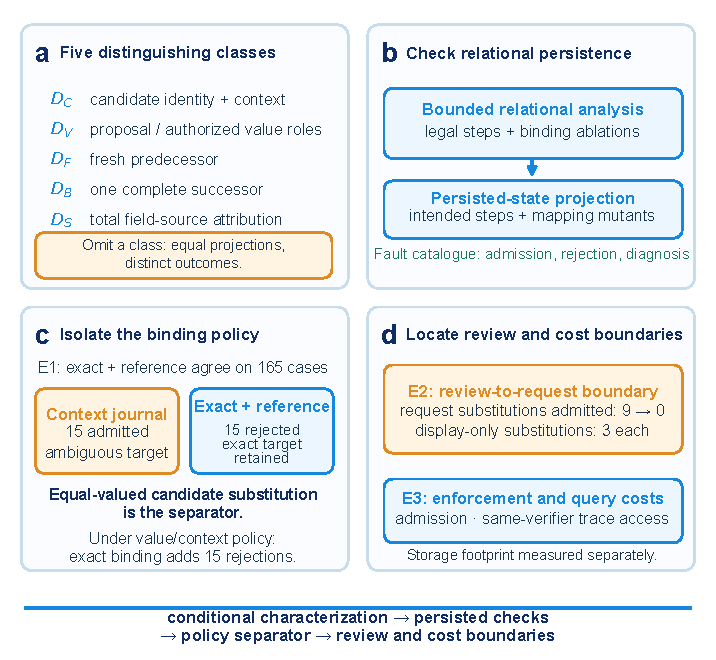
\includegraphics[width=0.975\textwidth]{figures/refined/figure-2-evidence-route.pdf}
\caption{Evidence route from the conditional characterization to persistence checks and E1--E3. E1 supplies the policy separator; E2 tests request binding and the presentation boundary; E3 characterizes enforcement and query costs. Displayed E1/E2 results are read from archived tables; timing totals are checked against CSV summaries. Diagram scripting assisted by OpenAI Codex}
\label{fig:evidence-route}
\end{figure}

\subsection{RQ1: rich-context and exact-binding comparison}

A separately written \code{sqlite3} journal retains immutable candidates/events, review context, versions, transactions, and complete field sources. Its \emph{context} configuration checks field, version, evidence, and retained context while omitting candidate/certificate identifiers and instance-creation time. Its \emph{exact} configuration adds the reviewed-candidate link. The third arm invokes the reference's actual transaction. We score both instance authorization and the looser value/context policy.

Fifteen inputs cross eleven case families and three mechanisms. Twelve deterministically selected archived proposal cells contain four distinct values; three synthetic type controls bring the total to seven. They enter newly constructed histories, rather than complete historical-task replays. Cases exercise Accept, Correction, multi-field admission, equal-valued candidate and different-evidence substitutions, staleness, replay, unauthorized value, and three interrupted transaction locations. Online Resource 1, Section S6 lists the inputs and cases.

After acceptance, an independent reader checks six provenance questions on three fields: proposal, authorized value, reviewer, reviewed candidate, current value, and source version. Each accepted history contributes eighteen answers, classified as correct, wrong, ambiguous, or unavailable. Rejection requires the expected reason and unchanged logical fact-database digest, measured after authorization preparation. Prior review records may persist. Original strengthened-baseline continuity checks have a separate denominator.

\subsection{RQ2: review-to-confirmation boundary}

Local Chrome/Playwright runs an instrumented review fixture backed by \code{ReviewForms.confirm}. An independent driver records the displayed candidate, proposal, and authorized value before confirmation. Three JSON inputs cross ten interactions and two paths, giving sixty cases; six confirmations separately prepare replay setups. Positive controls cover acceptance, correction, and reselection. Candidate/value/principal request substitutions, stale/replayed requests, interrupted commits, and display-only substitution probe distinct boundaries.

The original path is compared with a server-held session binding candidate, version, reviewer, and value. Acceptance, agreement with recorded review intent, and writes on rejection are recorded. The fixture uses fixed principal labels and a separate session database. The resulting request and presentation boundaries are interpreted in \cref{sec:discussion}.

\subsection{RQ3: current-version costs}

Two ten-cell admission comparisons contribute 4,000 observations each; a 36-cell trace comparison contributes 14,400. Each cell has five warmups and 200 timed calls per arm in seeded randomized order, for 22,400 timed observations excluding warmups. Environment versions and full grids are in Online Resource 1, Sections S1, S4, and S6.

The mechanism comparison times complete confirmation on shared recognition-source workloads. Construction and database cloning are excluded: the journal opens its connection before timing, whereas the reference may connect lazily inside confirmation. The study measures these complete call boundaries; \cref{sec:discussion} explains their implementation differences.

A separate manual-source materialization ablation times persistence of a prevalidated delta while retaining authority rows, complete sources, transactionality, and CAS. Its result must match the precomputed relational fingerprint. Validation and planning occur outside that timer; its full-path column belongs to a different workload from the mechanism comparison.

The trace comparison holds the verifier fixed and changes three bulk repository reads to identifier enumeration and point lookups. Every returned complete object must agree. The grid varies record width, history length, and total records. Storage fixtures populate full/reduced schemas at three transition scales; their footprint excludes external evidence/model outputs, and the reduced schema has fewer audit obligations.

\section{Results}
\label{sec:results}

\subsection{RQ1: exact binding and persisted conformance}

\paragraph{E1: equal-valued candidate separation}
\label{sec:executable-relation-result}
Fifteen equal-valued candidate substitutions separated the authorization policies. The context journal accepted all 15: their values and retained context satisfied its policy, although the admitted instances differed from the reviewed targets. Both exact-binding mechanisms rejected them. The exact journal and relational reference agreed on all 165 paired decisions and query-answer sets. All mechanisms rejected substitutions with different retained evidence.

% Source: DKE-supplement/tables/e1-comparison.csv; exact fields retained.
\begin{table}[tb]
\centering
\small
\caption{E1: 165 executions per mechanism. Instance violations are accepted cases violating the instance policy. Extra rejections are rejected cases valid under the value/context policy. Query counts refer to field-level answers after acceptance. All arms had zero value/context-policy violations and zero rejections with fact writes.}
\label{tab:dke-comparator}
\setlength{\tabcolsep}{4pt}
\begin{tabularx}{\linewidth}{@{}Xrrrrr@{}}
\toprule
 & Accepted & Instance & Extra & \multicolumn{2}{c}{Query answers} \\
Mechanism & cases & violations & rejections & Correct & Ambiguous \\
\midrule
Context journal & 60 & 15 & 0 & 1,020 & 60 \\
Exact journal & 45 & 0 & 15 & 810 & 0 \\
Reference & 45 & 0 & 15 & 810 & 0 \\
\bottomrule
\end{tabularx}
\end{table}


The separator concerns the required authorization target. Under instance accountability, the rejected substitutions are unauthorized; under the looser value/context policy, the exact mechanisms make 15 additional rejections. Thus the experiment isolates a policy choice rather than treating context approval as inherently incorrect.

All 495 executions completed without harness errors. Each exact mechanism accepted 45 legal cases and rejected 120 without fact-database writes after authorization preparation, including all three rollback locations.

Accepted context-journal histories produced 1,020 correct answers and sixty ambiguous reviewed-candidate answers. Each exact mechanism produced 810 correct answers and none wrong, ambiguous, or unavailable. Totals reflect eighteen answers per accepted history, with more acceptances under the context policy. The ambiguous answers expose the same instance distinction after commit.

The original strengthened-baseline continuity run reproduced seven-of-eight single-history agreement, with equal-valued substitution as the separator; its paired-history distinction is a separate ninth check. The richer exact journal closes that gap in E1 by preserving the authorization link. The evaluated relation is therefore enforceable in both storage designs.

\paragraph{Formal and persisted support}
All 72 Alloy outcomes matched the manifests, with legal, ablation, source-attack, and nonempty-precondition witnesses in both profiles. The checked assertions had no counterexamples within scope. The intended projections were satisfiable, and the mapping mutants were unsatisfiable. Every catalogue case, both stateful profiles, and all 33 rollback/concurrency tests passed in the retained execution.

The illustrative lifecycle retained proposal 100, separately authorized correction 101, exact sources for the other two fields, and a complete trace/export. Six archived AI-origin lifecycles and ten pinned-interface controls also matched their outcomes. The new execution passed 85 selected regressions and ten harness checks. These are separate evidence layers; the retained tests were not all rerun for E1--E3.

\subsection{RQ2: request binding and display controls}

The server-held gate rejected all nine request substitutions that the original path accepted despite disagreement with recorded review intent. Both paths accepted three display-only substitutions. Request binding therefore separates request-to-review consistency from presentation integrity.

% Source: DKE-supplement/tables/e2-cases.csv, grouped by case family and mode.
\begin{table}[tb]
\centering
\small
\caption{E2: accepted cases by interaction family, with three JSON values per named interaction. Each path has thirty cases; replay setup is additional. All nine original-path rejections and eighteen gate rejections made zero fact writes.}
\label{tab:dke-review}
\begin{tabularx}{\linewidth}{@{}Xrrr@{}}
\toprule
Interaction family & Cases/path & Original & Session gate \\
\midrule
Accept, Correction, reselection & 9 & 9 & 9 \\
Candidate, value, principal request substitutions & 9 & 9 & 0 \\
Stale, replay, precommit interruption & 9 & 0 & 0 \\
DOM-only substitution & 3 & 3 & 3 \\
\midrule
All cases & 30 & 21 & 12 \\
\bottomrule
\end{tabularx}
\end{table}


Each path completed thirty browser cases and accepted all nine legitimate controls. Both rejected stale submissions, replays, and precommit interruptions without fact writes. In the display-only controls, the page showed B while server and request continued with A. The original transaction preserves the caller-supplied binding; the gate additionally checks it against the earlier server-held review record.

\subsection{RQ3: admission, trace, and storage costs}

\paragraph{Admission}
Both admission comparisons completed ten cells. Shared mechanism queries agreed; materialized states matched their precomputed fingerprints. \Cref{tab:dke-admission-selected} shows representative cells; Online Resource 1, Section S4 retains every cell.

% Sources: DKE-supplement/tables/e3-mechanism-summary.csv and e3-ablation-summary.csv.
\begin{table}[tb]
\centering
\footnotesize
\caption{Representative E3 admission cells: p50/p95 (ms), 200 observations per arm/cell. Recognition and manual-source columns use separate workloads; prevalidated timing excludes validation and planning. All ten cells are in Online Resource 1, Section S4.}
\label{tab:dke-admission-selected}
\setlength{\tabcolsep}{3pt}
\begin{tabular}{@{}rr r r r r@{}}
\toprule
 & & \multicolumn{2}{c}{Recognition-source mechanisms} & \multicolumn{2}{c}{Manual-source ablation} \\
\cmidrule(lr){3-4}\cmidrule(l){5-6}
Fields & Changed & Reference & Exact journal & Full & Prevalidated \\
\midrule
1 & 1 & 28.79/50.50 & 10.40/13.32 & 23.23/33.76 & 9.97/14.63 \\
32 & 32 & 187.24/292.72 & 13.07/17.77 & 122.68/200.00 & 13.89/22.61 \\
128 & 128 & 712.00/1039.83 & 22.09/30.53 & 427.59/621.20 & 23.50/37.43 \\
\bottomrule
\end{tabular}
\end{table}


With 128 fields all changed, median reference confirmation was 712.00~ms and exact-journal confirmation 22.09~ms. Both enforce exact binding; these are complete-call costs for the compared implementations. In the separate manual-source ablation, full confirmation was 427.59~ms and prevalidated materialization 23.50~ms. The latter times persistence after validation and planning, as defined in \cref{sec:evaluation}.

\paragraph{Reverse trace}
All 36 paired cells completed 14,400 calls with identical full returned objects. At 128 fields, 100 versions, and 1,000 records, bulk p50/p95 was 170.24/216.75~ms versus 509.09/595.85~ms for point access, a median ratio of 2.99.

% Source: DKE-supplement/tables/e3-trace-summary.csv, fields=128 and records=1000.
\begin{table}[tb]
\centering
\small
\caption{E3 trace: representative cells with 128 fields and 1,000 total records. Latencies are p50/p95 milliseconds; each arm has 200 timed observations per row. SQL counts are constant within each row and arm. The complete 36-cell grid is deposited.}
\label{tab:dke-trace}
\begin{tabular}{@{}rrrrr@{}}
\toprule
 & \multicolumn{2}{c}{Latency (ms)} & \multicolumn{2}{c}{SQL statements} \\
\cmidrule(lr){2-3}\cmidrule(l){4-5}
Versions & Bulk & Point reads & Bulk & Point reads \\
\midrule
1 & 28.68/43.26 & 209.81/256.03 & 12 & 396 \\
10 & 39.69/48.16 & 233.82/285.43 & 12 & 423 \\
100 & 170.24/216.75 & 509.09/595.85 & 12 & 693 \\
\bottomrule
\end{tabular}
\end{table}


Bulk tracing used twelve SQL statements in every measured cell; the largest point-access cell used 693. With the same current verifier in both arms, the result attributes the measured difference to repository access. The constant statement count concerns round trips; field and history processing still contribute to total work.

\paragraph{Schema footprint}
Full-schema sizes were 1.52, 13.16, and 134.53~MiB at the tested transition scales, with roughly 1.1~kB incremental main-database storage per transition relative to the reduced fixture.

% Source: DKE-supplement/tables/storage.csv; MiB=bytes/1048576.
\begin{table}[htbp]
\centering
\small
\caption{E3 synthetic schema footprint after checkpointing. Incremental bytes per transition equal the full-minus-reduced main-database size divided by transition count. External evidence files are excluded.}
\label{tab:storage-cost}
\begin{tabular}{@{}rrrr@{}}
\toprule
Transitions & Full (MiB) & Reduced (MiB) & Incremental bytes/transition \\
\midrule
1,000 & 1.52 & 0.48 & 1085.4 \\
10,000 & 13.16 & 2.88 & 1077.2 \\
100,000 & 134.53 & 28.45 & 1112.3 \\
\bottomrule
\end{tabular}
\end{table}


These are database footprints for the full and reduced audit obligations defined in \cref{sec:evaluation}.

\subsection{Separate historical integration}
\label{sec:historical-integration}

The archived matrix retains 1,260 planned runs. Strict benign yield was 320/360 (88.89\%) and post-hoc endpoint yield 331/360 (91.94\%), with 25 unscorable runs; all 93 runtime failures remain recorded. Fixed host checks recorded no unauthorized mutation in 720 invalid-tuple calls or 179 capability-unavailable branches, the latter making no admission call. This reporting separates task completion from authority checks, analogous to AgentDojo's task/security outcomes \citep{debenedetti2024agentdojo}. The historical evidence supports restricted-interface integration separately from E1/E2; Online Resource 1, Section S5 preserves conditional denominators, configuration-specific failures, and annotation.

\section{Discussion and limitations}
\label{sec:discussion}

\subsection{What the results establish}

Correction-aware admission preserves the distinction between proposal origin and human value authority through commit. A reviewer can authorize 101 for a candidate that proposed 100; both values remain attributable to their respective roles. Total field sources then connect changed values to their authorization and preserve unchanged fields' exact earlier sources. The resulting history answers questions that the final value alone leaves unresolved.

The policy comparison isolates the reviewed instance within that history. Rich retained context can identify the permitted content while leaving more than one candidate consistent with it. Exact binding preserves the particular target: the journal and reference agree on all 165 corresponding decisions and query-answer sets, while 15 substitutions separate them from context approval. The policies differ in the granularity of accountability. Applications requiring instance accountability must preserve that link even when candidate content is equivalent.

The five paired histories show how missing information can conceal a failure. Alloy checks the encoded admission steps, and persisted-state projections test whether the implementation follows them. E2 then checks the transfer from review to confirmation; E3 measures the calls and trace access needed to enforce and query the relation.

\subsection{Trust and validity boundaries}

The server-held gate establishes request-to-review consistency for the tested substitutions. Display-only controls identify the remaining presentation boundary. Host authentication, review-channel integrity, principal policy, hashing/canonicalization, and database execution remain trusted. Lineage establishes recorded authorization and sources; factual truth requires independent validation. Evidence checks compare stored hashes and locators rather than re-reading external bytes. Detecting external replacement therefore requires immutable storage or additional integrity checks. Commit-entry policy revalidation also leaves later-revoked in-flight operations able to commit (Online Resource 1, Section S2).

The model conditions and class-wise scope of Proposition 1 are specified in \cref{sec:contract}. Alloy checks finite scopes; \cref{sec:conformance} states the selected-projection boundary and the formal no-op, schema-uniqueness, and trace-prefix differences. Distributed revocation, other database engines, deletion/redaction, and retention expiry require additional design and evidence.

E1 reuses seven distinct proposal values in constructed cases, and the journals are same-study implementations. E2 uses a local scripted fixture, fixed principals, and separate session/fact databases. Human attention, hostile hosts, and cross-database crash atomicity require separate study. Historical hosted-agent outcomes and author-involved annotation have distinct scoring, missingness, and failure records in Online Resource 1, Section S5.

E3 characterizes one machine with uncontrolled background activity. The admission arms differ in schema, ORM, validation, functionality, and connection lifecycle. Their measured costs therefore do not isolate exact-binding overhead. The separate materialization ablation excludes validation/planning and is not a complete admission path. The paired trace study holds the verifier fixed; its constant SQL count leaves processing, prefix traversal, and memory free to grow with history and fields. Storage fixtures exclude external evidence/model outputs and compare different audit obligations. Online Resource 1, Sections S4, S6, and S7 retain the complete workload and validity details.

\subsection{Applying the relation}

Adoption begins with the approval policy and one correction traced through persisted records. Identify the reviewed candidate, authorized value, predecessor check, and changed/unchanged source links. Retain a legal control and a failure probe for each boundary. Online Resource 1, Section S3 provides the worked example and inspection checklist.

The relation can be enforced in relational tables or event journals by preserving these objects and validating their bindings together. Concrete post-initial admission creates transitions for changed values; renewed review or re-attribution without a value change belongs to a separate review-event path. An independently implemented deployment with operational reviewers would provide the next test of transferability.

\section{Conclusion}
\label{sec:conclusion}

An authoritative correction must preserve what the machine proposed and what the human authorized as distinct historical roles. Equal values and equivalent retained context do not make different persisted candidates the same authorization target. We specify a correction-aware admission relation that carries the reviewed instance and explicit authorized value through a fresh predecessor into an atomic complete successor with total field sources.

Five paired histories establish class-wise irredundancy in the declared observation model. Formal analysis, selected persisted-state projections, and transaction checks connect that characterization to executable enforcement. The exact-binding event journal and relational reference agree on all 165 corresponding cases, demonstrating the relation across both storage designs; equal-valued substitution isolates their policy difference from context approval.

The review-session study locates the request and presentation boundaries, while current-version workloads characterize admission and provenance reconstruction costs. Together, the results preserve original proposals through Correction, enforce the specified authorization target at commit, and keep each successor field's authorization and source queryable afterward.

\section*{Statements and Declarations}

\subsection*{Data and software availability}

The study uses synthetic and public lifecycle inputs. The new comparison, browser-boundary, and current-version cost evidence is deposited with code, raw receipts, database snapshots, screenshots, dependency locks, and manifests at \href{https://github.com/lhh666-6/auto-dete/tree/2645e5e18c900ea91c9c980e44195dc71e410432/DKE-supplement}{the frozen experiment archive}. The reference implementation is fixed at commit \code{c6d512843c905cab6d8521dd8c914f7fb26d85ae}, under \code{latest/code/implementation-fixed}. Its formal models, observation witnesses, and earlier annotation and integration evidence are accessible from \href{https://github.com/lhh666-6/auto-dete/tree/c6d512843c905cab6d8521dd8c914f7fb26d85ae/latest}{the frozen formal and historical evidence archive}. Historical v8 evidence remains separately versioned under commit \code{abcdb817835a2c0953e5a26d854f34d99347dc6a}. Online Resource 1, Section S1 maps the evidence layers and describes restoration of the losslessly compressed large database. Inspecting the deposit and reproducing the three new experiments requires no paid model calls; repeating historical hosted-agent runs requires provider credentials.

\subsection*{Ethics approval and consent to participate}

The new experiments use constructed data and scripted browser interactions, with no new human participants. In the historical annotation study, one author (X.W.) and one non-author volunteer independently coded benign completion outcomes; L.H. adjudicated the inter-human disagreement and separately reviewed eleven human--rule disagreements against the strict-trajectory criterion. X.W. also completed the textual-acknowledgment annotation. Only pseudonymous annotator identifiers were collected; both benign-endpoint coders were informed of the task and data use, and the non-author coder participated voluntarily. Annotation evaluated generated outputs rather than annotator characteristics. The authors assessed this activity as not requiring ethics approval. No animal subjects were involved.

\subsection*{CRediT authorship contribution statement}

Liang Hanghao: Conceptualization, Methodology, Software, Formal analysis, Investigation, Data curation, Validation, Visualization, Project administration, Writing--original draft, and Writing--review \& editing.

Xuan Wentao: Methodology, Formal analysis, Investigation, Data curation, Validation, Visualization, and Writing--review \& editing.

Chen Qile: Investigation and Validation.

Peng Peng: Supervision and Writing--review \& editing.

\subsection*{Funding}

This research received no external funding.

\subsection*{Competing interests}

The authors declare no competing interests.

\subsection*{AI-assisted preparation}

The authors used DeepSeek, OpenAI Codex, and Claude for code, analysis checks, literature organization, and manuscript and diagram preparation. OpenAI image generation supplied a design prototype for Figure 1; its model/version was not recorded. The final diagrams were rendered from scripts using Matplotlib 3.10.8. The authors verified sources, results, and figure content and take responsibility for the article.

\subsection*{Supplementary information}

Online Resource 1 contains the artifact guide, formal observation and projection details, worked correction example, full workload grids, and historical integration and validity records.



\bibliographystyle{sn-basic}
\bibliography{filtered}
\end{document}
